\label{motivations}
\subsection{Motivations}
The motivation for this project stems from previous courses I have taken such as `Fundamentals of Computer Architecture`, `Microcontrollers` and `Operating Systems`. When taking these course I really enjoyed the challenges behind working within an ARM based environment, such as working with few `variables` and having no pre-made software available to you. For me, these challenges raised the question of how viable it is to write an operating system for a microcontroller.
While I had done a simple form of this for my Microcontrollers course, I wanted to take it further by implementing more complex features. In addition to this I wanted to improve upon the work I had done. This work had been relatively rushed and messy as I was having to learn on the go, and I did not have much time to re-factor. From this I derived two main goals for this project; I wanted to develop an OS which was better structured, and I wanted to develop some sort of process management service for the ARM chip. The operating systems course should help with the development of the process management service, as the notes I have explain how operating systems manage processes and threads within an OS. This project is more concerned with developing threads rather than processes, the distinction being that a thread is usually a segment of a program running as a process. 

Finding ways of keeping my work organised became a large part of this project for me. Most of my programming experience has, until now, been focused on higher level languages such as C\# and Java. Due to this, developing for a low level language felt quite jarring due to the following characteristics of ARM, program structure can become disorganised and hard to read without self-imposed discipline; Braces and indentation are not enforced, which would usually expose the control flow of the program; Automated type checking does not exist. These problems reinforced the necessity of commenting in all my code, even beyond ARM. Consistently commenting an a specific style also became a key strategy to ensuring my code was readable. I often found myself trading off readability against efficiency.

\subsection{Background}
The system I built has it roots in the Microcontroller's course, and it derives much of its environment from the work done there. The system was built for the graphical debugger named `Komodo` \cite{kmd}. This acts as a `front end` for `back end` processor models. In my case the model I used was  and emulator called `Jimulator`. It provides me with the assembler for my ARM code, as well as the ability to load and run the assembled code on a virtual ARM processor. The debugging facilities it provides allow me to pause the code at breakpoints I set and inspect the state of the processors memory and registers. My working environment also consists of a few plug-ins for Jimulator. These plug-ins are as follows:

\begin{itemize}
	\item An 8 bit clock-based timer exposed as a byte in memory.
	\item 3 x 4 Virtual keypad with an interface set-up in the memory.
	\item A 320px x 240px virtual RGB display with an interface set-up in the memory of the arm chip.
\end{itemize}

These plug-ins for the Jimulator emulator expose themselves at static memory addresses with various interfaces.
The timer appears as a read-only memory location at 0xF100\_1010. This timer is free-running and increments at 1kHz. 
The keypad simulates a matrix keypad. It works by allowing the arm processor to activate scan lines and read the resulting input to determine which keys have been pressed. It also appears as a single byte containing both the scan-line bits, and the resulting output bits.

\begin{figure}[ht!]
	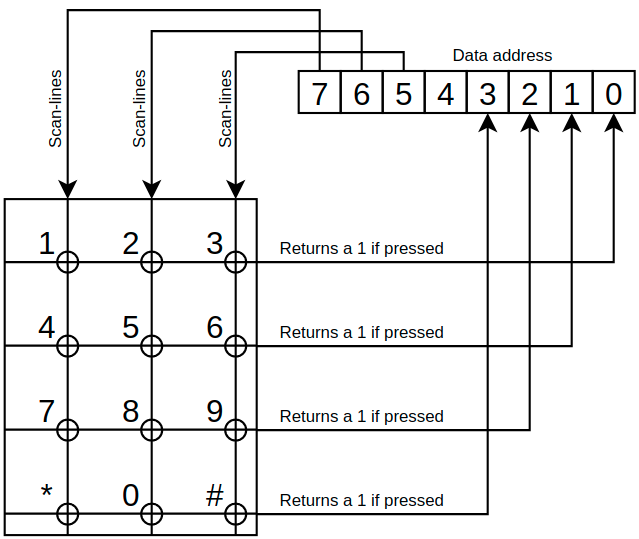
\includegraphics[width=0.5\linewidth]{figures/keypad.png}\centering
	\caption{Keypad Matrix Setup}
	\label{fig:keypad}
\end{figure}

The virtual screen is made of a vscreen program, connected to the Jimulator via a plug-in. The plug-in exposes the access to the screen via a frame buffer set-up in memory starting at 0xAC00\_0000. The memory set-up consists of 3 bytes for each pixel running left to right, top to bottom. The 3 bytes represent the RGB values of the corresponding pixel

\begin{figure}[ht!]
	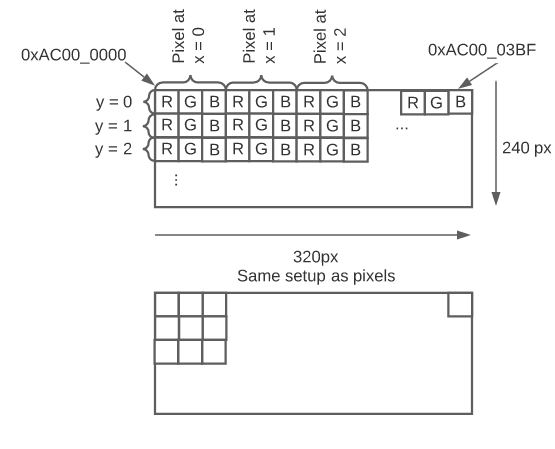
\includegraphics[width=0.5\linewidth]{figures/LCD.png}\centering
	\caption{Frame buffer memory set-up}
	\label{fig:LCDMem}
\end{figure}

The system I created required me to modify this starting environment by replacing the keypad with an new plug-in, which created and handled a new virtual keyboard as detailed later in \autoref{chap:virtualKeyboard}. 
